\documentclass{article}
\usepackage{float,amsmath}
\usepackage{graphicx}
\usepackage{color}
\usepackage[letterpaper,margin=1in]{geometry}
\usepackage{hyperref}

\usepackage{outlines}
\usepackage{enumitem}
\setenumerate[1]{label=\arabic*.}
\setenumerate[2]{label=\alph*.}
\setenumerate[3]{label=\arabic*.}
\setenumerate[4]{label=\roman*.}

\usepackage{cleveref}
\crefformat{footnote}{#2\footnotemark[#1]#3}
 
\begin{document}

\author{HERA Software Team}
\title{Correlator Specification Tradeoffs}
\maketitle

\setcounter{section}{-1}
\section*{Executive Summary}

\newpage

\section*{Introduction}
The specifications for the HERA correlator and real time processing (RTP) have important implications for science with HERA, 
particularly for image-based calibration, foreground subtraction and power spectra. 
These specifications also drive the data rate of HERA, and therefore the time and costs associated with processing and storing the data.

The effect on imaging and related activities is driven by the amount of decorrelation of the visibilities caused by integrating in time and frequency. 
Decorrelation causes \textit{baseline-dependent} changes in the instrument response (effective primary beam) that are challenging to model and will 
limit the accuracy of image-based calibration and foreground subtraction, which rely on high-quality visibility simulations. 

This memo explores trade-offs along four primary axes:

\begin{enumerate}
\item \textbf{Number of Frequency Channels}: Since the bandwidth is fixed (50-250 MHz), the number of channels is directly related to the channel 
width. Larger numbers of channels (narrower channel widths) lead to lower decorrelation and higher data rates.
The number of channels in the current correlator is 2048 (122kHz wide channels).
\item \textbf{Integration Time}: The final length of the integrations written by the correlator (after fringe-stopping if that is being done, see next item). 
Longer integration times lead to more decorrelation and lower data rates. The integration time of the current correlator is 10s.
\item \textbf{Fringe Stopping}: Fringe stopping removes the first-order decorrelation effect from integrating in time by phasing each visibility (at a very 
high time cadence, e.g. 100ms) to a fixed point on the celestial sphere before the final time integration step. Fringe stopping significantly decreases 
the decorrelation for a fixed final integration time. Fringe stopping has no effect on the data rate, but it requires more sophisticated firmware on the 
correlator (to handle the phasing). The current correlator does not do fringe stopping.
\item \textbf{Baseline Dependent Averaging}: Baseline dependent averaging refers to a practice of averaging baselines for longer times depending on 
their fringe-rate, with integration times selected to be integer factors of the correlator integration time that keep the visibility below some specified 
level of decorrelation. This means that the decorrelaton on short baselines will be \textit{increased} relative to doing no baseline dependent 
averaging, but it leads to a substantial decrease in the final data rate for HERA, which is dominated by short baselines. Baseline dependent 
averaging would be implemented in RTP, not the correlator, so it would not decrease the correlator data rate but it would decrease the data rate after 
RTP. Software adjustments would be required to handle baseline dependent averaging in down-stream code, but the software team is optimistic that 
most of the handling for it could be done in \texttt{pyuvdata} in a way that reduced the impact on most users. The current RTP does not do baseline 
dependent averaging.
\end{enumerate}

The plots and tables shown in this memo were produced using code and notebooks located in the 
ProjectFiles repository\footnote{\label{code_link} \url{https://github.com/HERA-Team/ProjectFiles/tree/master/spec_calcs}}. 
Interested parties are encouraged to run their own scenarios.

\begin{figure}
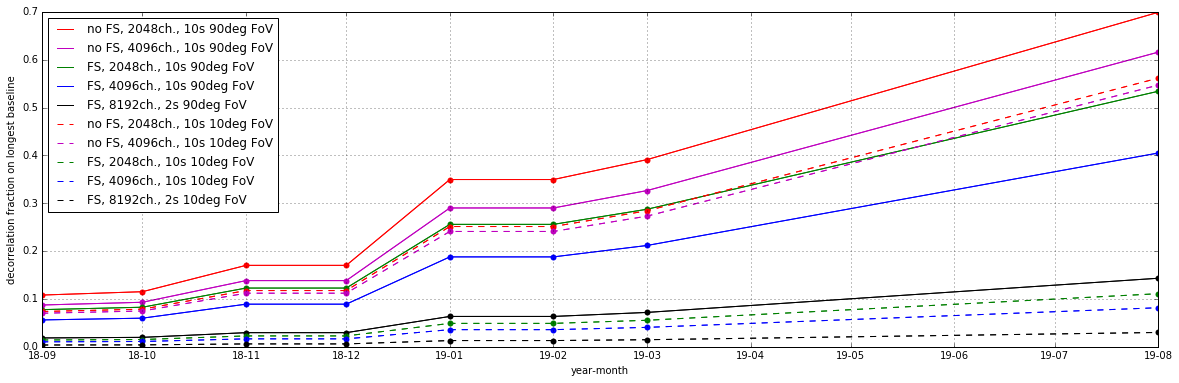
\includegraphics[width=\textwidth]{spec_calcs/decorrelation.png} 
\caption{Decorrelations on the longest baseline over the course of the buildout for various correlator options. The red line shows the current 
correlator specifications (2048 channels, 10s integration, no fringe stopping), the blue line shows the imaging-driven specifications 
(4096 channels, 10s integations with fringe stopping) for h2c and the magenta and green lines give two intermediate options. 
Finally, the black line shows an aggressive imaging-driven specification for the full array (8192 channels, 2s integrations with fringe stopping). 
Solid lines show the decorrelation at the horizon while the dashed lines show the decorrelation 10 degrees away from the zenith. 
This plot is generated in the  \texttt{h2c\_stats.ipynb} notebook\cref{code_link}.}
\label{Fig:decorr}
\end{figure}

\begin{figure}
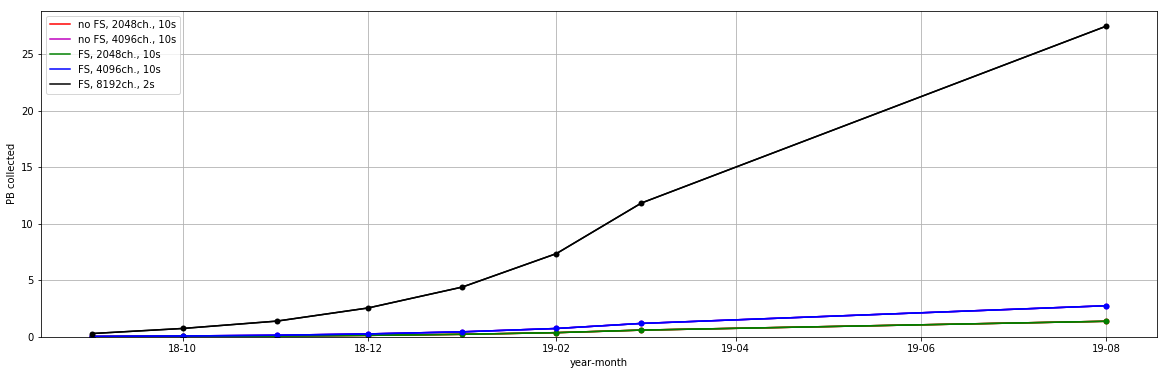
\includegraphics[width=\textwidth]{spec_calcs/corr_data_vols.png} 
\caption{Correlator data volumes on the longest baseline over the course of the buildout for various correlator options. 
The line colors are the same as in \ref{Fig:decorr}, but the green line is on top of the red line and the blue line is on top of the magenta line
because the data rate depends only on the number of frequency channels and the final integration time (not on fringe stopping). 
The data volumes after RTP can be decreased substantially by baseline-dependent averaging.
This plot is generated in the  \texttt{h2c\_stats.ipynb} notebook\cref{code_link}.}
\label{Fig:corr_vol}
\end{figure}



\end{document}